\section{Árvores}

\begin{frame}
	\begin{block}{Árvores Binárias de Busca}
		\begin{itemize}
			\item São estruturas de dados que permitem inserções, deleções e busca em complexidade logarítmica. 

			\item $O(\log n)$ para inserir, atualizar, deletar e buscar	
			
			\item É uma estrutura recursiva onde cada Nó contém outros dois nós, denominados filhos.

		\end{itemize}
	\end{block}
\end{frame}

\begin{frame}
	\begin{block}{Árvores Binárias de Busca}
		\begin{itemize}
			\item Esse tipo de estrutura de dados segue uma regra simples, os filhos da esquerda devem ser menores que seu pai. Os filhos da direita devem ser maiores que seu pai.

			\item Em outras palavra, ao inserir um novo nó devemos procurar a posição correta desse na árvore
		\end{itemize}
	\end{block}
\end{frame}

\begin{frame}
	\begin{block}{Árvores Binárias de Busca}
		\begin{figure}[!htb]
			\centering	  				
			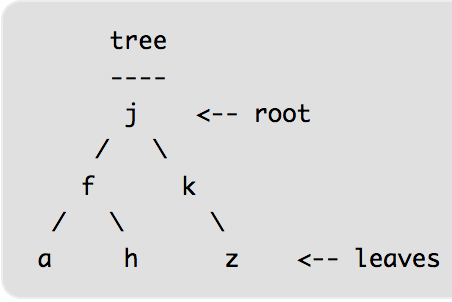
\includegraphics[height=3cm, width = 9cm]{./pic/arvoreCompletaComun.png}
			\caption{Exemplo de árvore binária de busca \cite{GEEKS_2018}}
		\end{figure}
	\end{block}
\end{frame}


\begin{frame}
	\begin{block}{Árvores Binárias de Busca}
		\begin{itemize}
			\item Algumas propriedades das árvores binárias:

			\item O número máximo de nós no nível $i$ é dado por: $2^{i-1}$ Nível aqui é o número de nós entre a raiz e o nó em questão
			
			\item A altura da árvore é $\log_{2} n$
			
			\item Uma árvore binária de altura $h$ tem no máximo $2^{h} -1$ nós
		\end{itemize}
	\end{block}
\end{frame}

\begin{frame}
	\begin{block}{Árvores Binárias de Busca}
		\begin{itemize}
			\item Exemplo de árvore balanceada completa:
		\end{itemize}
		\begin{figure}[!htb]
			\centering	  				
			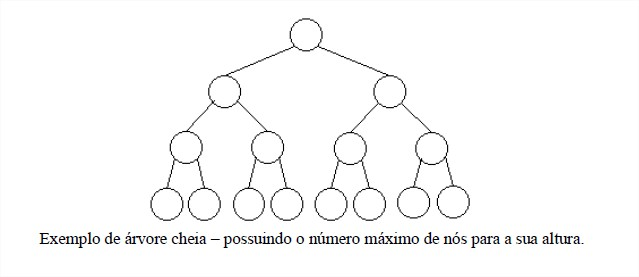
\includegraphics[height=3cm, width = 9cm]{./pic/arvoreCompleta.jpg}
			\caption{Exemplo de árvore balanceada \cite{GEEKS_2018}}
		\end{figure}
	\end{block}
\end{frame}


\begin{frame}
	\begin{block}{Árvores Binárias de Busca}
		\begin{itemize}
			\item Exemplo de árvore desbalanceada:
		\end{itemize}
		\begin{figure}[!htb]
			\centering	  				
			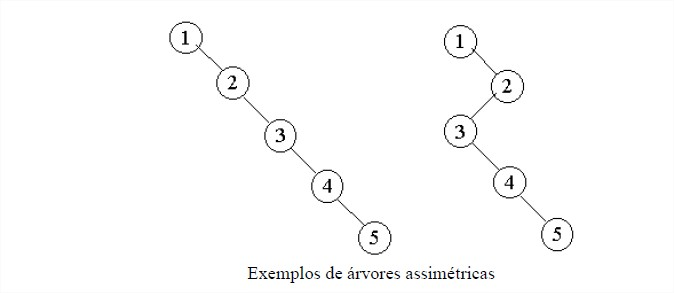
\includegraphics[height=3cm, width = 9cm]{./pic/arvoresAssimetricas.jpg}
			\caption{Exemplo de árvore desbalanceada \cite{GEEKS_2018}}
		\end{figure}
	\end{block}
\end{frame}


\begin{frame}
	\begin{block}{Árvores Binárias de Busca}
		\begin{itemize}
			\item Para percorrer árvores binárias de busca, temos três opções de percurso:

			\item Em ordem
			
			\item Pré-ordem
			
			\item Pós-ordem
		\end{itemize}
		\begin{figure}[!htb]
			\centering	  				
			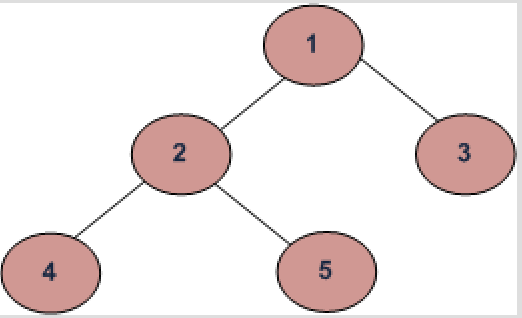
\includegraphics[height=3cm, width = 9cm]{./pic/passeioArvore.png}
			\caption{Exemplo de árvore \cite{GEEKS_2018}}
		\end{figure}
	\end{block}
\end{frame}

\begin{frame}
	\begin{block}{Imprime em Ordem}
		\begin{itemize}
			\item Exemplo de árvore para percorrermos:
			\item Inorder (Left, Root, Right) : 4 2 5 1 3
		\end{itemize}
			\begin{figure}[!htb]
			\centering	  				
			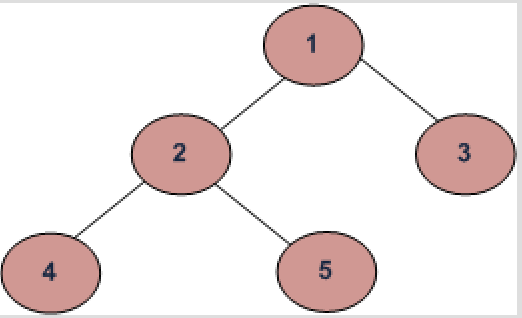
\includegraphics[height=3cm, width = 9cm]{./pic/passeioArvore.png}
			\caption{Exemplo de árvore \cite{GEEKS_2018}}
		\end{figure}
			\end{block}
\end{frame}
			
\begin{frame}[fragile]
	\begin{block}{}
		Imprimir árvore em ordem:
				\inputminted[linenos,
									fontsize=\footnotesize,
									baselinestretch=1.2,
									framesep=2mm,
									bgcolor=bg_gray, 
									frame=lines]
									{csharp}
									{./secoes/Arvores/imprimeEmOrdem.cs}
	\end{block}
\end{frame}
			
\begin{frame}
	\begin{block}{Imprime Pós-Ordem}
		\begin{itemize}
			\item Exemplo de árvore para percorrermos:
			\item Inorder (Left, Root, Right) : 4 5 2 3 1
		\end{itemize}
			\begin{figure}[!htb]
			\centering	  				
			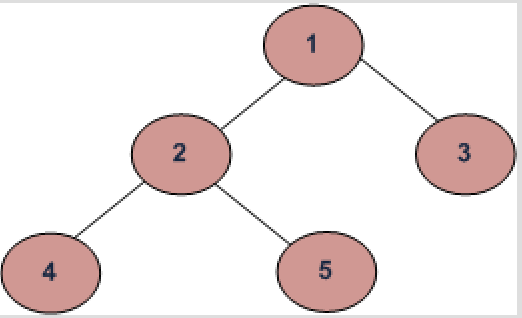
\includegraphics[height=3cm, width = 9cm]{./pic/passeioArvore.png}
			\caption{Exemplo de árvore \cite{GEEKS_2018}}
		\end{figure}
			\end{block}
\end{frame}

\begin{frame}[fragile]
	\begin{block}{}
		Imprimir árvore pós-ordem:
				\inputminted[linenos,
									fontsize=\footnotesize,
									baselinestretch=1.2,
									framesep=2mm,
									bgcolor=bg_gray, 
									frame=lines]
									{csharp}
									{./secoes/Arvores/imprimePosOrdem.cs}
	\end{block}
\end{frame}


\begin{frame}
	\begin{block}{Imprime Pré-Ordem}
		\begin{itemize}
			\item Exemplo de árvore para percorrermos:
			\item Inorder (Left, Root, Right) : 1 2 4 5 3
		\end{itemize}
			\begin{figure}[!htb]
			\centering	  				
			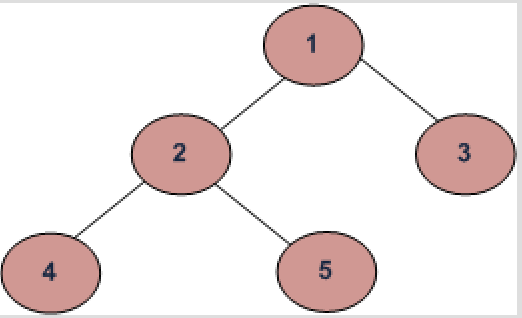
\includegraphics[height=3cm, width = 9cm]{./pic/passeioArvore.png}
			\caption{Exemplo de árvore \cite{GEEKS_2018}}
		\end{figure}
			\end{block}
\end{frame}

\begin{frame}[fragile]
	\begin{block}{}
		Imprimir árvore pré-ordem:
				\inputminted[linenos,
									fontsize=\footnotesize,
									baselinestretch=1.2,
									framesep=2mm,
									bgcolor=bg_gray, 
									frame=lines]
									{csharp}
									{./secoes/Arvores/imprimePreOrdem.cs}
	\end{block}
\end{frame}

\begin{frame}
	\begin{block}{Árvores Binárias de Busca}
		\begin{itemize}
			\item Para pesquisar em árvores:

			\item Compare a chave pesquisada com a raiz, se for menor vá para a direita, caso contrário vá para a esquerda. 
			
			\item Repita o processo novamente até encontrar o nó pesquisado ou chegar em uma folha e não encontrar o valor.
		\end{itemize}
	\end{block}
\end{frame}

\begin{frame}
	\begin{block}{Imprime Pré-Ordem}
		\begin{itemize}
			\item Simular no quadro a pesquisa pela chave: "7":
		\end{itemize}
			\begin{figure}[!htb]
			\centering	  				
			\includegraphics[height=3cm, width = 9cm]{./pic/BSTSearch.png}
			\caption{Exemplo de árvore \cite{GEEKS_2018}}
		\end{figure}
			\end{block}
\end{frame}


\begin{frame}
	\begin{block}{Imprime Pré-Ordem}
		\begin{itemize}
			\item Como inserir valores?

			\item Percorra a árvore até encontrar a folha que será pai do novo nó.
			
			\item Insira uma nova folha na árvore e acerte os ponteiros.
		\end{itemize}
	\end{block}
\end{frame}

\begin{frame}
	\begin{block}{Imprime Pré-Ordem}
		\begin{itemize}
			\item Exemplo de inserção do valor: "40" na árvore:
		\end{itemize}
		\begin{figure}[!htb]
			\centering	  				
			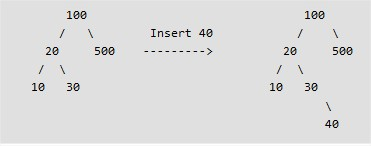
\includegraphics[height=3cm, width = 9cm]{./pic/insercao.jpg}
			\caption{Exemplo de árvore \cite{GEEKS_2018}}
		\end{figure}
	\end{block}
\end{frame}


\begin{frame}
	\begin{block}{Imprime Pré-Ordem}
		\begin{itemize}
			\item Como podemos deletar nós? Temos três casos de deleção:

			\item Deletar uma folha
			
			\item Nó para ser deletado tem apenas um filho
			
			\item Nó para ser deletado tem dois filhos
		\end{itemize}
	\end{block}
\end{frame}


\begin{frame}
	\begin{block}{Imprime Pré-Ordem}
		\begin{itemize}
			\item Deletar uma folha, simplesmente delete (caso simples)
		\end{itemize}
		\begin{figure}[!htb]
			\centering	  				
			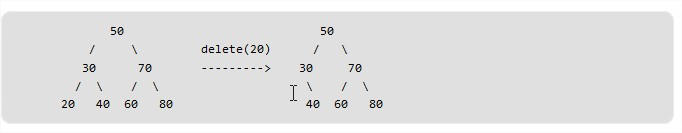
\includegraphics[height=3cm, width = 9cm]{./pic/delecao1.jpg}
			\caption{Exemplo de árvore \cite{GEEKS_2018}}
		\end{figure}
	\end{block}
\end{frame}

\begin{frame}
	\begin{block}{Imprime Pré-Ordem}
		\begin{itemize}
			\item Deletar nó com apenas um filho, troque o valor do filho com o pai, e delete o filho (com valor trocado).
		\end{itemize}
		\begin{figure}[!htb]
			\centering	  				
			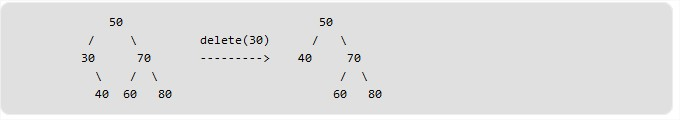
\includegraphics[height=3cm, width = 9cm]{./pic/delecao2.jpg}
			\caption{Exemplo de árvore \cite{GEEKS_2018}}
		\end{figure}
	\end{block}
\end{frame}

\begin{frame}
	\begin{block}{Imprime Pré-Ordem}
		\begin{itemize}
			\item Deletar nó com dois filhos, encontre o sucessor em ordem, troque seus valores com  o pai e delete o sucessor (com valor trocado)
		\end{itemize}
		\begin{figure}[!htb]
			\centering	  				
			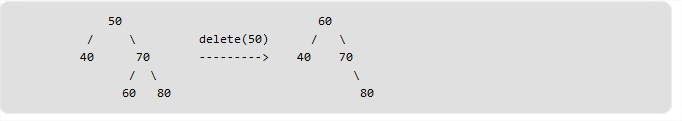
\includegraphics[height=3cm, width = 9cm]{./pic/delecao3.jpg}
			\caption{Exemplo de árvore \cite{GEEKS_2018}}
		\end{figure}
	\end{block}
\end{frame}

\begin{frame}
	\begin{block}{Exemplo de deleção}
		\begin{figure}[!htb]
			\centering	  				
			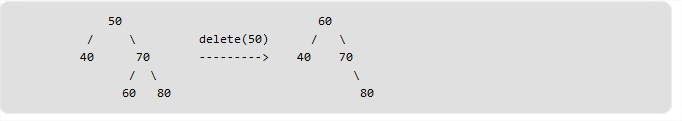
\includegraphics[height=3cm, width = 9cm]{./pic/delecao3.jpg}
			\caption{Exemplo de árvore \cite{GEEKS_2018}}
		\end{figure}
	\end{block}
\end{frame}

\begin{frame}
	\begin{block}{Exemplo de deleção}
		\begin{figure}[!htb]
			\centering	  				
			\includegraphics[height=3cm, width = 9cm]{./pic/BSTDelete.png}
			\caption{Exemplo de árvore \cite{GEEKS_2018}}
		\end{figure}
	\end{block}
\end{frame}

\begin{frame}
	\begin{block}{Exemplo de deleção}
		\begin{figure}[!htb]
			\centering	  				
			\includegraphics[height=3cm, width = 9cm]{./pic/BSTDelete-2.png}
			\caption{Exemplo de árvore \cite{GEEKS_2018}}
		\end{figure}
	\end{block}
\end{frame}

\begin{frame}
	\begin{block}{AVL}
		\begin{itemize}
			\item Percebemos que manter a árvore balanceada é um desafio. Se a árvore desbalancear podemos cair no caso de uma busca sequencial em lista ligada.
			
			\item Como garantir que a árvore não vai ficar desbalanceada?
			
			\item Para garantir isso existe a estrutura denominada AVL, é uma árvore binária de busca com as mesmas regras que já estudamos. Porém há uma vantagem, ela se auto balanceia a cada inserção em tempo $\log n$
		\end{itemize}
	\end{block}
\end{frame}


\begin{frame}
	\begin{block}{AVL}
		\begin{itemize}
			\item A diferença principal aqui é que sempre que inserimos ou deletamos precisamos avaliar se ocorreu um desbalanceamento. Se ocorreu, precisamos rebalancear a árvore.

			\item Existem quatro casos de rotação que podemos aplicar, dependendo do caso de inserção.
		\end{itemize}
	\end{block}
\end{frame}

\begin{frame}
	\begin{block}{Rotação: Left Left}
		\begin{itemize}
			\item Left Left
		\end{itemize}
		\begin{figure}[!htb]
			\centering	  				
			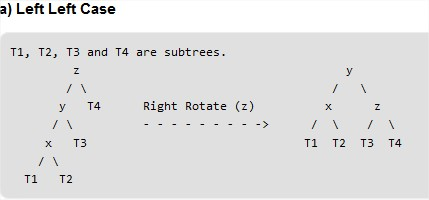
\includegraphics[height=3cm, width = 9cm]{./pic/leftleft.jpg}
			\caption{Exemplo de rotação left - left \cite{GEEKS_2018}}
		\end{figure}
	\end{block}
\end{frame}


\begin{frame}
	\begin{block}{Rotação: Left Rigth}
		\begin{itemize}
			\item Left Rigth
		\end{itemize}
		\begin{figure}[!htb]
			\centering	  				
			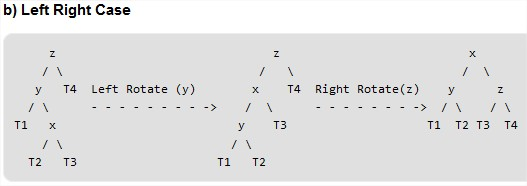
\includegraphics[height=3cm, width = 9cm]{./pic/leftRigth.jpg}
			\caption{Exemplo de rotação left - rigth \cite{GEEKS_2018}}
		\end{figure}
	\end{block}
\end{frame}

\begin{frame}
	\begin{block}{Rotação: Rigth Rigth}
		\begin{itemize}
			\item Rigth Rigth
		\end{itemize}
		\begin{figure}[!htb]
			\centering	  				
			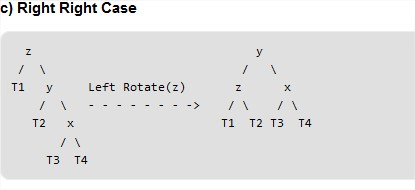
\includegraphics[height=3cm, width = 9cm]{./pic/rigthrigth.jpg}
			\caption{Exemplo de rotação right - rigth \cite{GEEKS_2018}}
		\end{figure}
	\end{block}
\end{frame}

\begin{frame}
	\begin{block}{Rotação: Rigth Left}
		\begin{itemize}
			\item Rigth Left
		\end{itemize}
		\begin{figure}[!htb]
			\centering	  				
			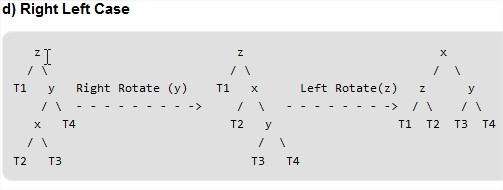
\includegraphics[height=3cm, width = 9cm]{./pic/rigthLeft.jpg}
			\caption{Exemplo de rotação right - left \cite{GEEKS_2018}}
		\end{figure}
	\end{block}
\end{frame}

\begin{frame}
	\begin{block}{AVL}
		\begin{itemize}
			\item Como determinar o caso de inserção de uma árvore com raiz "z" novo nó "w" ?
			
			\item Simples:
			
			\item y é o filho da esquerda de z e x é o filho da esquerda de y(LL)
			\item y é o filho da esquerda de z e x é o filho da direita de y(LR)
			\item y é o filho da direita de z e x é o filho da direita de y(RR)
			\item y é o filho da direita de z e x é o filho da esquerda de y(RL)
		\end{itemize}
	\end{block}
\end{frame}


\begin{frame}
	\begin{block}{Rotação: Rigth Left}
		\begin{figure}[!htb]
			\centering	  				
			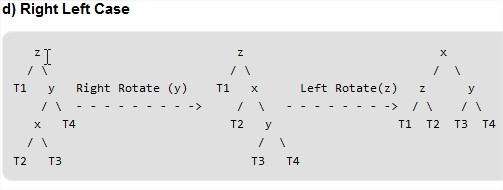
\includegraphics[height=4cm, width = 10cm]{./pic/rigthLeft.jpg}
			\caption{Exemplo de rotação right - left  \cite{GEEKS_2018}}
		\end{figure}
	\end{block}
\end{frame}


\begin{frame}
	\begin{block}{Exemplo de inserção}
		\begin{figure}[!htb]
			\centering	  				
			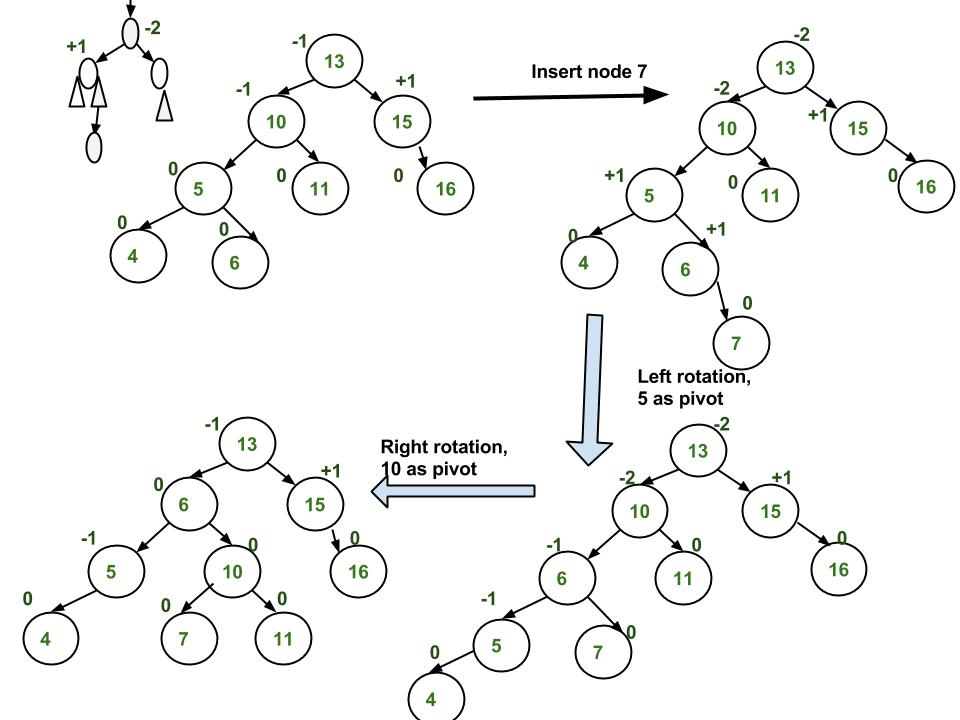
\includegraphics[height=6cm, width = 10cm]{./pic/AVL_exemplo_01.jpg}
			\caption{Exemplo de inserção  \cite{GEEKS_2018}}
		\end{figure}
	\end{block}
\end{frame}

\begin{frame}
	\begin{block}{Exemplo de inserção}
		\begin{figure}[!htb]
			\centering	  				
			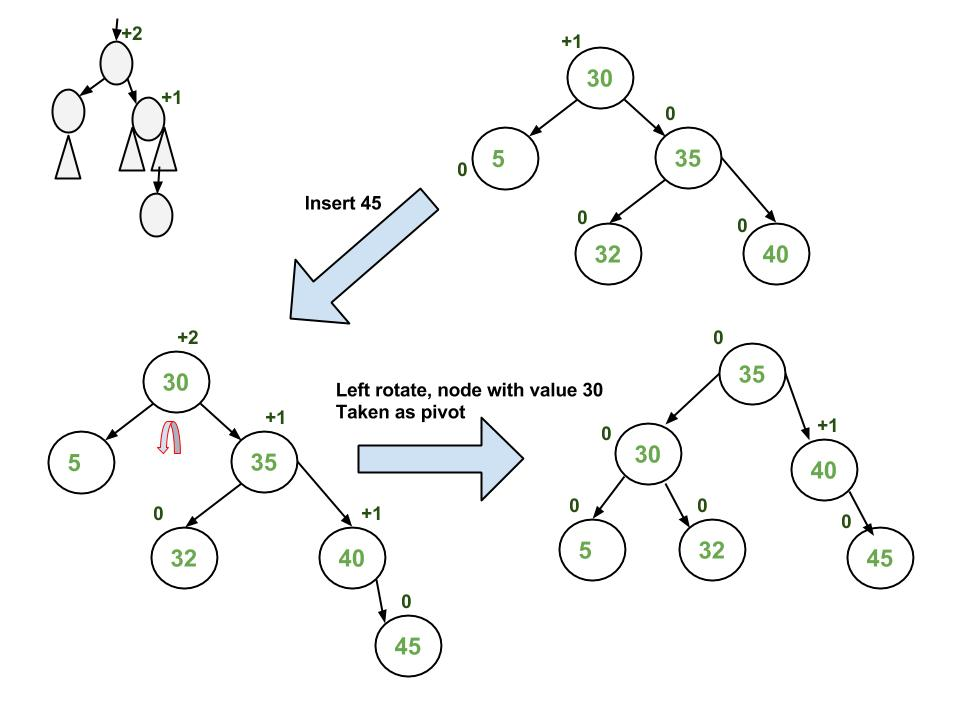
\includegraphics[height=6cm, width = 10cm]{./pic/AVL_exemplo_02.jpg}
			\caption{Exemplo de inserção  \cite{GEEKS_2018}}
		\end{figure}
	\end{block}
\end{frame}

\begin{frame}
	\begin{block}{Exemplo de inserção}
		\begin{figure}[!htb]
			\centering	  				
			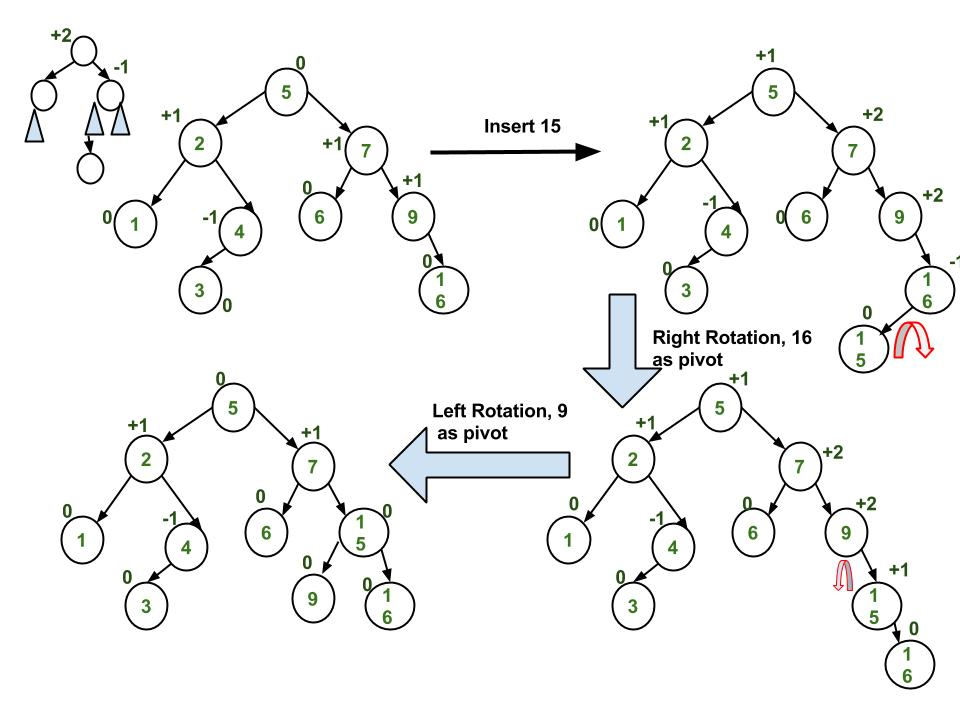
\includegraphics[height=6cm, width = 10cm]{./pic/AVL_exemplo_03.jpg}
			\caption{Exemplo de inserção  \cite{GEEKS_2018}}
		\end{figure}
	\end{block}
\end{frame}

\begin{frame}
	\begin{block}{Exemplo de inserção}
		\begin{figure}[!htb]
			\centering	  				
			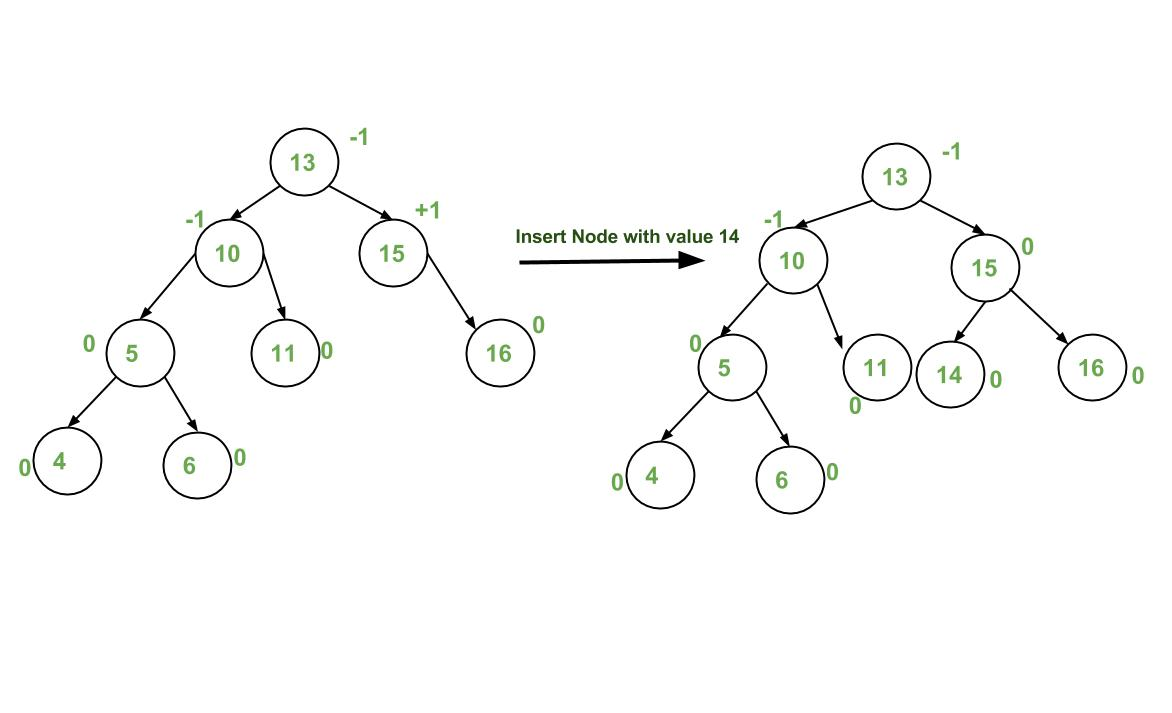
\includegraphics[height=6cm, width = 10cm]{./pic/AVL_exemplo_04.jpg}
			\caption{Exemplo de inserção  \cite{GEEKS_2018}}
		\end{figure}
	\end{block}
\end{frame}

\begin{frame}
	\begin{block}{Exemplo de inserção}
		\begin{figure}[!htb]
			\centering	  				
			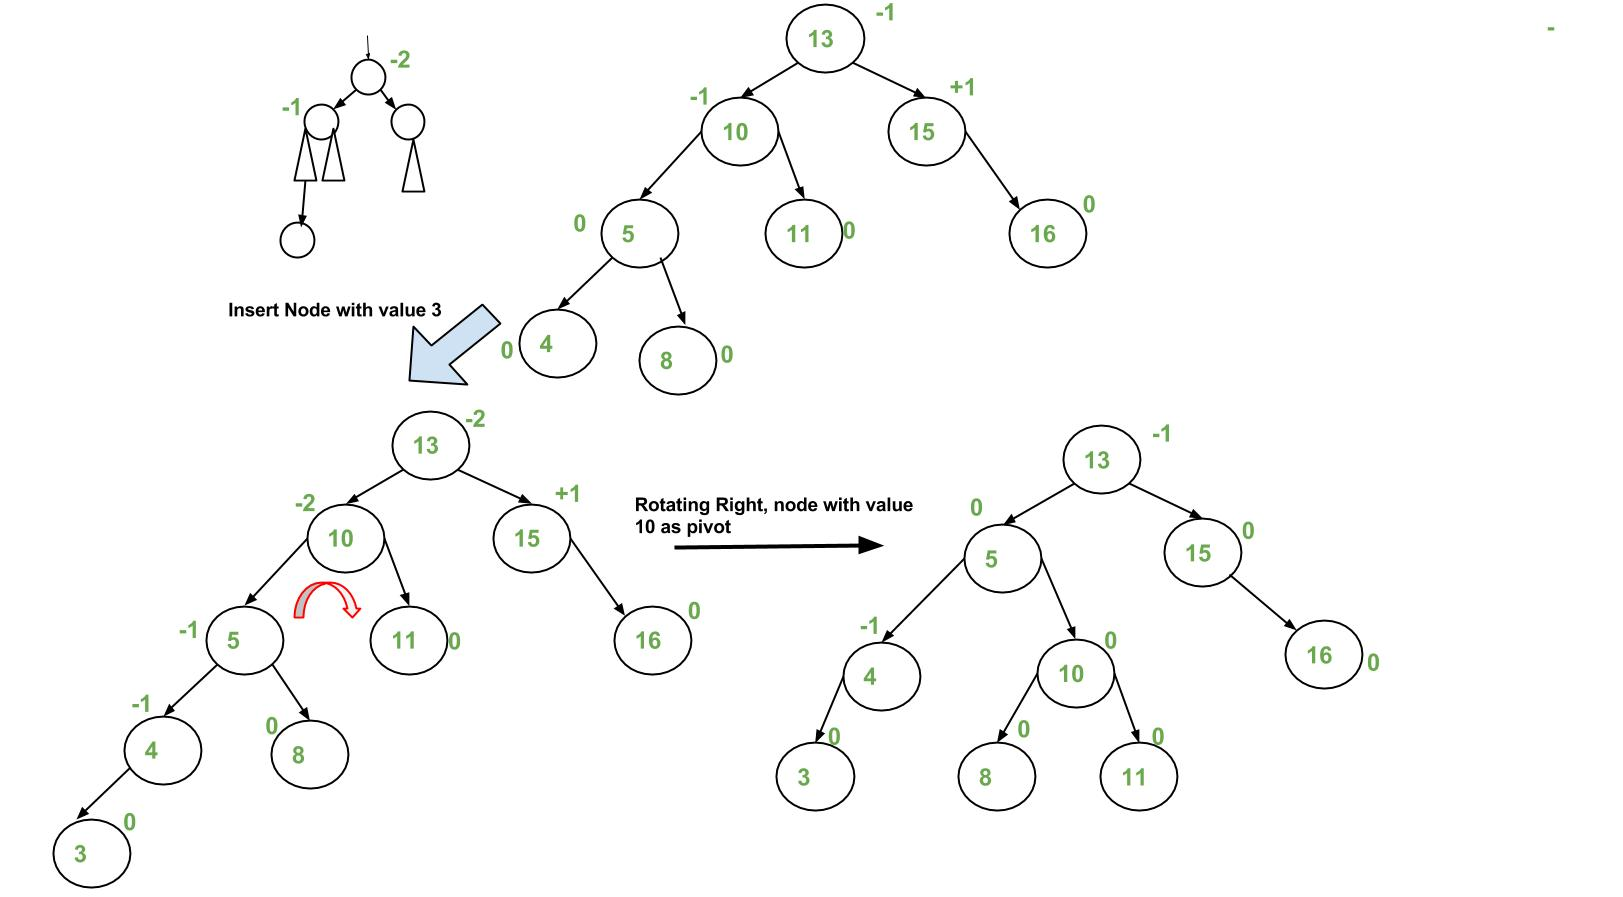
\includegraphics[height=6cm, width = 10cm]{./pic/AVL_exemplo_05.jpg}
			\caption{Exemplo de inserção  \cite{GEEKS_2018}}
		\end{figure}
	\end{block}
\end{frame}

